\documentclass[a4paper,12pt,twoside]{article}
\usepackage[left=1in,right=1in,top=1in,bottom=1in]{geometry}

\usepackage{xeCJK}
\setCJKmainfont{Songti TC}
\setCJKfamilyfont{kai}{Songti TC}
\newcommand{\kai}{\CJKfamily{kai}} % 用 \kai{使用楷書}

\usepackage{lmodern}
\usepackage{titling}
\usepackage{titlesec}
\usepackage{graphicx}
\usepackage{float}
\usepackage{amsmath, amsthm, amssymb, amsfonts, mathrsfs}
\usepackage{upgreek} % 直立的希臘字母

\usepackage[shortlabels]{enumitem}
\usepackage{setspace}
\renewcommand{\baselinestretch}{1.5}
\usepackage[colorlinks]{hyperref}
\usepackage{fancyvrb}
\usepackage{fancyhdr}
\usepackage{multicol}
\usepackage{caption}
\usepackage{listings}
\usepackage{bm}
\usepackage{bbm} % for \mathbbm{1} (indicator function)
\usepackage{centernot}
\usepackage{mdframed}
\usepackage{tikz}
\usetikzlibrary{patterns, arrows.meta, positioning}
\usepackage[nameinlink, capitalise]{cleveref}
\usepackage{diagbox}
\usepackage{booktabs}
\usepackage{multirow,array}
\usepackage{tabularx}
\usepackage{mathtools}
\usepackage{indentfirst} % 首段 indent
\setlength{\parindent}{2em}
\usepackage{cancel} % 數學式子畫線槓掉
\newcommand\mcancel[2][red]{\setbox0=\hbox{$#2$}%
\rlap{\raisebox{.45\ht0}{\textcolor{#1}{\rule{\wd0}{1pt}}}}#2}
\usepackage{datetime2}

\AtBeginDocument{%
 \setlength{\abovedisplayskip}{6pt}
 \setlength{\belowdisplayskip}{6pt}
 \setlength{\abovedisplayshortskip}{4pt}
 \setlength{\belowdisplayshortskip}{4pt}
}

\definecolor{codegreen}{rgb}{0,0.6,0}
\definecolor{codegray}{rgb}{0.5,0.5,0.5}
\definecolor{codepurple}{rgb}{0.58,0,0.82}
\definecolor{backcolour}{rgb}{0.95,0.95,0.92}

\lstdefinestyle{mystyle}{
 backgroundcolor=\color{backcolour},
 commentstyle=\color{codegreen},
 keywordstyle=\color{magenta},
 numberstyle=\tiny\color{codegray},
 stringstyle=\color{codepurple},
 basicstyle=\ttfamily\footnotesize,
 breakatwhitespace=false,
 breaklines=true,
 captionpos=b,
 keepspaces=true,
 numbers=left,
 numbersep=5pt,
 showspaces=false,
 showstringspaces=false,
 showtabs=false,
 tabsize=2
}
\lstset{style=mystyle}

\hypersetup{citecolor=blue, linkcolor=blue, urlcolor=blue}

\DeclareMathOperator{\supp}{supp}
\DeclareMathOperator{\skewness}{Skewness}
\DeclareMathOperator{\DU}{D-U}
\DeclareMathOperator{\CU}{C-U}
\DeclareMathOperator{\Geo}{Geo}
\DeclareMathOperator{\Pois}{Pois}
\DeclareMathOperator{\Gam}{Gam}
\DeclareMathOperator{\LN}{LogN}
\DeclareMathOperator{\cov}{Cov}
\DeclareMathOperator*{\argmax}{arg\,max}
\DeclareMathOperator*{\argmin}{arg\,min}
\DeclareMathOperator{\re}{Re}
\DeclareMathOperator{\im}{Im}

\newcommand{\N}{\mathbb{N}}
\newcommand{\Z}{\mathbb{Z}}
\newcommand{\Q}{\mathbb{Q}}
\newcommand{\R}{\mathbb{R}}
\newcommand{\C}{\mathbb{C}}
\newcommand{\G}{\mathcal{G}}
\newcommand{\mP}{\mathbb{P}}
\newcommand{\F}{\mathcal{F}}
\newcommand{\B}{\mathcal{B}}
\newcommand{\1}{\mathbbm{1}}
\newcommand{\Poi}{\text{Poi}}
\newcommand{\Var}{\text{Var}}
\newcommand{\as}{\text{a.s.}}
\newcommand{\vect}[1]{\boldsymbol{\mathbf{#1}}}
\newcommand{\paren}[1]{\left({#1}\right)}
\newcommand{\brk}[1]{\left[{#1}\right]}
\newcommand{\curl}[1]{\left\{{#1}\right\}}
\renewcommand{\lambda}{\lambdaup}

\theoremstyle{definition} % 定理環境 style 改用正體
\newtheorem{theorem}{定理}
\newtheorem{definition}{定義}
\newtheorem*{definition*}{定義}
\newtheorem{example}{例子}
\newtheorem{exercise}{練習}
\newtheorem{corollary}{推論}
\newtheorem{property}{性質}
\newtheorem{prop}{命題}
\newtheorem{lemma}{引理}
\newtheorem{problem}{問題}
\newtheorem*{remark}{註}

\renewcommand{\figurename}{圖}
\renewcommand{\tablename}{表}

\DeclareMathOperator{\var}{Var}
\DeclareMathOperator{\corr}{corr}
\DeclareMathOperator{\rank}{rank}
\DeclareMathOperator{\MSE}{MSE}
\DeclareMathOperator{\SSE}{SSE}
\DeclareMathOperator{\SST}{SST}
\DeclareMathOperator{\SSR}{SSR}
\DeclareMathOperator{\sgn}{sign}
\DeclareMathOperator{\alt}{Alt}
\DeclareMathOperator{\adj}{adj}
\DeclareMathOperator{\curlOp}{curl}
\DeclareMathOperator{\spn}{span}
\DeclareMathOperator{\sse}{SSE}
\DeclareMathOperator{\tr}{tr}

\newcommand{\ep}{\varepsilon}
\newcommand{\p}{\partial}
\newcommand{\abs}[1]{\left|#1\right|}
\newcommand\norm[1]{\left\lVert#1\right\rVert}
\newcommand{\innerprod}[1]{\langle#1\rangle}
\newcommand{\ds}{\displaystyle}
\newcommand{\blank}{\rule[-1mm]{1.5cm}{0.1mm}}
\newcommand{\dint}{\displaystyle\int}
\renewcommand{\bar}{\overline}

\newtheoremstyle{remark}{}{}{}{}{\bfseries\sffamily}{.}{.5em}{#1}
\theoremstyle{remark}

\newtheorem*{remark*}{\textit{Remark}}
\newtheorem*{solution*}{解}

\AtEndEnvironment{solution*}{\hfill$\square$}
\newtheorem*{hint*}{Hint}


\newcommand{\redtext}[1]{{\color{red} #1}}
\newcommand{\bluetext}[1]{{\color{blue} #1}}

\fancypagestyle{firstpage}{
  \fancyhf{}
  \fancyhead[R]{\small《高中數學實驗教材》第 4 冊（自然組）}
  \fancyhead[L]{\small 第 2 章\quad 二次幾何\quad 第一部分：錐線的演變}
  \fancyfoot[C]{\thepage}
}

\pagestyle{fancy}
\setlength{\headheight}{14pt}
\renewcommand{\headrulewidth}{0.5pt}
\renewcommand{\footrulewidth}{0pt}
\fancyhead{}
\fancyhead[LE]{\small 《高中數學實驗教材》第四冊（自然組）}
\fancyhead[RO]{\small 第二章\quad 二次幾何\quad 第一部分：錐線的演變}
\fancyfoot[C]{\thepage}

\title{\LARGE\textbf{《高中數學實驗教材》第四冊（自然組）}\\[0.5em] \Large\textbf{第二章\quad 二次幾何\quad 第一部分：錐線的演變}}
\author{\textbf{高中數學實驗教材編輯小組}\quad 編著}
\date{民國六十五年（1976）三版}

\begin{document}

\maketitle
\thispagestyle{firstpage}

% ==========================================
% 掃描檔勘誤、文字校訂與疑難處說明（依規則整理於目錄之前）
% ==========================================
\section*{【說明】第二章掃描檔勘誤、疑難處與文義校訂表}
\addcontentsline{toc}{section}{【說明】第二章掃描檔勘誤、疑難處與文義校訂表}
\label{sec:errata_notes_b4_ch2}

本章依據 1976 年三版《高中數學實驗教材 第四冊（自然組）》（高二下）第二章「二次幾何 第一部分：錐線的演變」掃描原件完整轉錄為 \LaTeX{} 格式。為忠實反映教材原始內容並兼顧排版品質與嚴謹性，依作業規範將掃描檔中出現之印刷訛誤、符號缺漏、字模損毀、歷史印記雜訊及文義疑難處詳細考證彙整於下表。讀者可點擊表格中之章節連結直接跳至正文對應位置：

\begin{table}[H]
\centering
\small
\renewcommand{\arraystretch}{1.35}
\begin{tabularx}{\textwidth}{|p{3.2cm}|p{3.8cm}|X|}
\hline
\textbf{章節位置} & \textbf{掃描檔原始現象 / 誤植} & \textbf{考證說明與校訂處理} \\ \hline

\hyperref[sec:b4-2-1]{§ II-1 頁 66 彗星軌道引述} & 
「受到其他星體的吸引而改鍵初衷」 & 
「改鍵」二字實為「改變」之排版訛字（鉛字「變」誤植為「鍵」）。正文予以校訂並備註。 \\ \hline

\hyperref[sec:b4-2-3]{§ II-3 頁 74 截面圖號體例} & 
插圖標為「圖 3-1」、「圖 3-2」等 & 
原書圖號採以小節號「§ II-3」作為首碼之歷史編排體例。正文忠實保留原刊編號並加註說明。 \\ \hline

\hyperref[sec:b4-2-4]{§ II-4 頁 79 丹德林雙球定理} & 
內切球切點與焦點一致性推導 & 
轉錄時以現代立體向量與 TikZ 向量繪圖高解析度重繪丹德林雙球模型，文字完全忠實原文。 \\ \hline

\hyperref[sec:b4-2-5]{§ II-5 頁 88 準線觀點選授標記} & 
目次標註「$\ddagger$ § II-5 準線觀點」 & 
原書目次加註「$\ddagger$」，正文章末附註標註「**」，依目次「注意 1」規範為選授進階幾何內容。 \\ \hline

\hyperref[note:b4-ch2-p96-appendix-note]{§ II-5 頁 96 章末附註三垂線證明} & 
定理 4 補充證明中 $AM \perp p$ & 
正文完整重現三垂線定理之立體幾何嚴格推導與作圖，補足正文論述之嚴謹性。 \\ \hline

\end{tabularx}
\caption{第二章掃描檔勘誤、疑難處與文義校訂表}
\label{tab:errata_b4_ch2}
\end{table}

\vspace{1em}
\hrule
\vspace{1em}

\tableofcontents
\newpage

% =========================================================================
% 《高中數學實驗教材》第四冊（自然組）
% 第二章 二次幾何 第一部分：錐線的演變
% =========================================================================

\section{二次幾何\texorpdfstring{\quad }{ }第一部分：錐線的演變}
\label{sec:b4-ch2}

\begin{center}
\begin{minipage}{0.75\textwidth}
\begin{itemize}[leftmargin=2em, itemsep=0.3em]
  \item[§ II-1] \textbf{引論}
  \begin{itemize}[leftmargin=2em, itemsep=0.2em]
    \item[甲、] 拋物線
    \item[乙、] 天體運動的軌跡：二次曲線
  \end{itemize}
  \item[§ II-2] \textbf{一個關於球的切線長度的事實}
  \item[§ II-3] \textbf{圓錐曲線}
  \item[§ II-4] \textbf{焦半徑與離心率的觀點}
  \item[$\ddagger$ § II-5] \textbf{準線觀點}
\end{itemize}
\end{minipage}
\end{center}

\begin{center}
$* \qquad * \qquad * \qquad * \qquad *$
\end{center}

本冊有三個章節討論二次幾何．所謂二次幾何，在代數上指的是二元二次方程式及其所相應的多項式；在幾何上則相應於圓，橢圓，拋物線，雙曲線等曲線．本章的重點是要從圓錐與平面的截痕出發，以純幾何的方式來觀察這四種曲線如何隨著截平面的變動而互相演變，並導出它們的幾何特徵性質（焦半徑性質與準線性質）．

% =========================================================================
% § II-1 引論
% =========================================================================
\subsection{引論}
\label{sec:b4-2-1}

\subsubsection*{甲、拋物線}

在初中我們已經學過二次函數
\begin{equation}
y = ax^2 + bx + c \quad (a \neq 0) \label{eq:b4-2-1-1}
\end{equation}
的圖形是一條拋物線．

在物理上，拋物線有非常廣泛的應用．例如地表附近的拋體運動，如果不計空氣阻力，質點的運動軌跡就是一條拋物線（圖 \ref{fig:b4-2-1-1}）．

\begin{figure}[H]
\centering
\begin{tikzpicture}[scale=0.9]
  \draw[thick, -Stealth] (-0.5, 0) -- (6, 0) node[right] {$x$};
  \draw[thick, -Stealth] (0, -0.5) -- (0, 3.5) node[above] {$y$};
  \filldraw (0, 0) circle (1.5pt) node[below left] {$O$};

  % Parabola projectile
  \draw[very thick, blue, domain=0:5, samples=50] plot (\x, {-0.4*(\x)*(\x - 5)});
  \draw[thick, -Stealth, red] (0, 0) -- (1.5, 2.0) node[above] {$\mathbf{v}_0$};
  \node at (2.5, 2.8) {\small 拋體運動軌跡};
\end{tikzpicture}
\caption{拋體運動之拋物線軌跡}
\label{fig:b4-2-1-1}
\end{figure}

又如光學上，為了探照燈或汽車前燈能將光線匯聚成一束平行光，又能射達遠處，我們可利用拋物面鏡，而將燈心放在焦點 $F$ 處（圖 \ref{fig:b4-2-1-2}）．這樣經鏡面反射的光線將平行射出，不致有漫射性的浪費，又可及於遠處．

\begin{figure}[H]
\centering
\begin{tikzpicture}[scale=0.95]
  % Parabolic mirror
  \draw[very thick, blue, domain=-2.6:2.6, samples=60] plot ({0.4*\x*\x}, \x);
  % Mirror backing hatching
  \foreach \y in {-2.4, -2.0, -1.6, -1.2, -0.8, -0.4, 0, 0.4, 0.8, 1.2, 1.6, 2.0, 2.4} {
    \draw[gray!60, thin] ({0.4*\y*\y}, \y) -- ++(-0.25, -0.15);
  }

  \coordinate (F) at (0.625, 0);
  \filldraw[red!80!black] (F) circle (2pt) node[below=3pt, fill=white, inner sep=1.5pt] {$F$ (焦點)};

  % Light rays with arrows
  \draw[thick, -Stealth, orange!90!black] (F) -- (1.6, 2.0);
  \draw[thick, -Stealth, orange!90!black] (1.6, 2.0) -- (5.0, 2.0);

  \draw[thick, -Stealth, orange!90!black] (F) -- (0.4, 1.0);
  \draw[thick, -Stealth, orange!90!black] (0.4, 1.0) -- (5.0, 1.0);

  \draw[thick, -Stealth, orange!90!black] (F) -- (0.4, -1.0);
  \draw[thick, -Stealth, orange!90!black] (0.4, -1.0) -- (5.0, -1.0);

  \draw[thick, -Stealth, orange!90!black] (F) -- (1.6, -2.0);
  \draw[thick, -Stealth, orange!90!black] (1.6, -2.0) -- (5.0, -2.0);

  % Axis
  \draw[dashed, gray!70] (0, 0) -- (5.2, 0) node[right] {\small 對稱軸};
\end{tikzpicture}
\caption{拋物面鏡之光學性質}
\label{fig:b4-2-1-2}
\end{figure}

在這一光學的應用中我們所採用的只是拋物線這種形狀本身，並不計較圖 \ref{fig:b4-2-1-1} 中它的位置．因此為了簡化，我們常將這拋物線的頂點平移到座標系的原點 $O$ 使呈右圖 \ref{fig:b4-2-1-3} 之形狀．此時 \eqref{eq:b4-2-1-1} 式因含 $(0, 0)$ 點，以 $x = 0$ 及 $y = 0$ 代入得 $c = 0$．又圖形對稱〔註〕於 $Y$ 軸，故 $b = 0$（見作業 1）．因此，\eqref{eq:b4-2-1-1} 式變成
\begin{equation}
y = ax^2 \label{eq:b4-2-1-1p}
\end{equation}
習慣上，我們考慮拋物線向兩側開口的情形，而以
\begin{equation}
y^2 = 4kx \label{eq:b4-2-1-1pp}
\end{equation}
表示，其中為了方便取係數為 $4k$，這 \eqref{eq:b4-2-1-1pp} 式常稱為拋物線的標準式（詳見 § III-3）．

\begin{figure}[H]
\centering
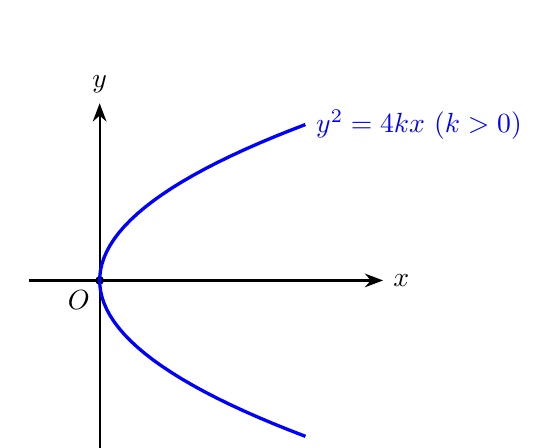
\begin{tikzpicture}[scale=0.9]
  \draw[thick, -Stealth] (-1, 0) -- (4, 0) node[right] {$x$};
  \draw[thick, -Stealth] (0, -2.5) -- (0, 2.5) node[above] {$y$};
  \filldraw (0, 0) circle (1.5pt) node[below left] {$O$};
  \draw[very thick, blue, domain=-2.2:2.2, samples=50] plot ({0.6*\x*\x}, \x) node[right] {$y^2 = 4kx$ ($k > 0$)};
\end{tikzpicture}
\caption{拋物線之標準方向}
\label{fig:b4-2-1-3}
\end{figure}

〔註〕在座標幾何中點 $(x, y)$ 對 $Y$ 軸的對稱點為 $(-x, y)$，其對 $X$ 軸的對稱點為 $(x, -y)$，若一點在一圖形上，其對稱點亦在其上，則稱此圖形對稱．又點 $(-x, -y)$ 為 $(x, y)$ 對於原點的對稱點，而若一圖形包含一點必包含此點對原點的對稱點，則稱此圖形對稱於原點．參考第一章作業 24．

\begin{example}[論例 1]
時常我們碰到的自然現象雖非二次函數，但用二次函數來估計比用一次函數估計精確．已知電壓與電流同時為 $0$，現在我們在電壓 $x = 1.2$ 伏特時，測得電流 $y = 0.8$ 毫安培，於是由直線 $y = \frac{0.8}{1.2}x = \frac{2}{3}x$，來估計電流與電壓間的關係（一次逼近，圖 \ref{fig:b4-2-1-4}a）．若要得到較精確的估計，可用二次函數（卽拋物線）$y = ax + bx^2$ 來估計它，這時要決定 $a, b$ 之值，我們就得做兩次實驗才夠，例如在電壓 $x = 2$ 伏特時，我們再次測得電流為 $1$ 毫安培．由
\[ \begin{cases} 0.8 = 1.2a + (1.2)^2 b \\ 1 = 2a + 2^2 b \end{cases} \]
求解 $a, b$ 得 $a = \frac{11}{12}, b = -\frac{5}{24}$，故在零點附近電流與電壓的關係可用下式估計：
\[ y = \frac{11}{12}x - \frac{5}{24}x^2 \approx 0.92x - 0.21x^2 \quad \text{（二次逼近，圖 \ref{fig:b4-2-1-4}b）} \]
若欲得更精確的估計，我們可用多項式 $y = a_1x + a_2x^2 + \dots + a_nx^n$ 來估計它，這時我們便須做 $n$ 次測量才能定出 $a_1, a_2, \dots, a_n$．
\end{example}

\begin{figure}[H]
\centering
\begin{subfigure}[b]{0.45\textwidth}
\centering
\begin{tikzpicture}[scale=1.1]
  \draw[thick, -Stealth] (-0.3, 0) -- (3, 0) node[right] {\small 電壓 $x$};
  \draw[thick, -Stealth] (0, -0.3) -- (0, 2) node[above] {\small 電流 $y$};
  \draw[very thick, blue] (0, 0) -- (2.5, 1.67) node[right] {\small $y = \frac{2}{3}x$};
  \filldraw (1.2, 0.8) circle (1.5pt) node[below right] {\small $(1.2, 0.8)$};
\end{tikzpicture}
\caption{一次逼近}
\end{subfigure}
\hfill
\begin{subfigure}[b]{0.45\textwidth}
\centering
\begin{tikzpicture}[scale=1.1]
  \draw[thick, -Stealth] (-0.3, 0) -- (3, 0) node[right] {\small 電壓 $x$};
  \draw[thick, -Stealth] (0, -0.3) -- (0, 2) node[above] {\small 電流 $y$};
  \draw[very thick, red, domain=0:2.5, samples=50] plot (\x, {0.92*\x - 0.21*\x*\x});
  \filldraw (1.2, 0.8) circle (1.5pt) node[below right] {\small $(1.2, 0.8)$};
  \filldraw (2.0, 1.0) circle (1.5pt) node[above] {\small $(2, 1)$};
\end{tikzpicture}
\caption{二次逼近}
\end{subfigure}
\caption{電流與電壓關係之一次與二次逼近}
\label{fig:b4-2-1-4}
\end{figure}

\subsubsection*{乙、天體運動的軌跡：二次曲線}

\eqref{eq:b4-2-1-1} 式 $y = ax^2 + bx + c$ 中，注意只有 $x$ 的最高次項二次項．如果我們考慮一般的二元二次方程式，亦卽式中亦可帶有 $y^2, xy$ 之項如
\begin{equation}
Ax^2 + 2Bxy + Cy^2 + Dx + Ey + F = 0 \label{eq:b4-2-1-2}
\end{equation}
（其中 $A, B, C, D, E, F$ 為實常數），則從這方程的軌跡〔稱為二次曲線〕，我們得到許多新的曲線，正是這些曲線使我們能夠妥善地描寫宇宙中一整套天體運動的軌跡及其他一些實際現象．同時透過對這些曲線的了解，我們在高中以後的課程裏將能探討二元二次函數的一些重要性質．

天體運動很多是週而復始的，這使我們很自然地想起圓．一個圓心為點 $A(a, b)$，半徑為 $r$ 的圓 $C$，其上（指圓周上）的點應是到 $A$ 的距離為定長 $r$ 的點，亦卽點 $P(x, y)$ 在 $C$ 上的充要條件是
\[ |PA| = r \iff |PA|^2 = r^2 \]
由畢氏定理知
\begin{equation}
(x - a)^2 + (y - b)^2 = r^2 \label{eq:b4-2-1-3}
\end{equation}
與甲段的理由一樣，如只注意圓的形狀本身可移 $A$ 點至原點 $O$，而得圓的標準式
\begin{equation}
x^2 + y^2 = r^2 \label{eq:b4-2-1-4}
\end{equation}
這是 \eqref{eq:b4-2-1-2} 式的一種特殊形式．

\begin{figure}[H]
\centering
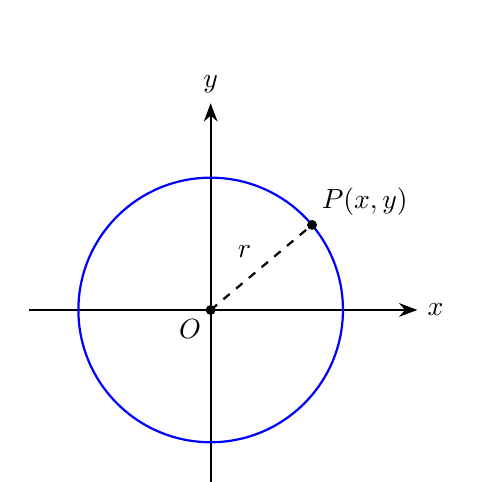
\begin{tikzpicture}[scale=1.05]
  \draw[thick, -Stealth] (-2.2, 0) -- (2.5, 0) node[right] {$x$};
  \draw[thick, -Stealth] (0, -2.2) -- (0, 2.5) node[above] {$y$};
  \draw[thick, blue] (0, 0) circle (1.6);
  \filldraw (0, 0) circle (1.5pt) node[below left] {$O$};

  \coordinate (P) at (40:1.6);
  \filldraw (P) circle (1.5pt) node[above right] {$P(x, y)$};
  \draw[thick, dashed] (0, 0) -- (P) node[midway, above left] {$r$};
\end{tikzpicture}
\caption{圓之幾何定義}
\label{fig:b4-2-1-5}
\end{figure}

那麼圓能否描寫週而復始的天體運動？由觀測及計算的結果我們發覺：卽使只看太陽系的行星運轉，若假定太陽位置固定，行星的軌跡並不正好是圓，一般時候是呈一個壓扁了的圓的形狀，卽所謂“橢圓”．若取適當正交座標系使扁的方向為 $Y$ 軸方向（上下方），凸的方向為 $X$ 軸方向（左右方），則它的方程式相當於“分別調整 $X$ 軸與 $Y$ 軸上的距離概念”而把 \eqref{eq:b4-2-1-4} 式變形如
\begin{equation}
\frac{x^2}{a^2} + \frac{y^2}{b^2} = 1 \quad (a, b > 0) \label{eq:b4-2-1-5}
\end{equation}
這式子的導引將另作詳述（§ III-1）．我們稱 \eqref{eq:b4-2-1-5} 式為橢圓的標準式．

\begin{figure}[H]
\centering
\begin{tikzpicture}[scale=1.05]
  \draw[thick, -Stealth] (-3, 0) -- (3, 0) node[right] {$x$};
  \draw[thick, -Stealth] (0, -2) -- (0, 2) node[above] {$y$};
  \draw[very thick, blue] (0, 0) ellipse (2.2 and 1.3);
  \filldraw (1.4, 0) circle (2pt) node[below=3pt, fill=white, inner sep=1pt] {$F$（太陽）};
  \filldraw (-1.4, 0) circle (2pt) node[below=3pt, fill=white, inner sep=1pt] {$F'$};
  \coordinate (P) at (-1.1, 1.12);
  \filldraw (P) circle (2pt) node[above left] {$P$（行星）};
  \draw[thick, dashed, red] (-1.4, 0) -- (P) -- (1.4, 0);
\end{tikzpicture}
\caption{克卜勒行星橢圓軌道與焦點}
\label{fig:b4-2-1-7}
\end{figure}

圖 \ref{fig:b4-2-1-7} 所示的行星運轉中，太陽的位置 $F$ 並不正好居中，$F$ 與其對 $Y$ 軸的鏡像點（或稱對稱點）$F'$ 合稱為橢圓的兩個焦點．這兩焦點的位置可從橢圓如下的特徵性質〔註〕求得：「橢圓上任意點 $P$ 到 $F$ 與 $F'$ 的距離和為一定長，亦卽 $|PF| + |PF'| = \text{定長}$」（見 § III-1）．

但上述週而復始的行星運行方式並不能概括所有的天體運動，比如有些彗星去而不返．當然其中一個可能原因是此星在太陽系外受到其他星體的吸引而改變初衷或消失無遺．但也有其他可能：比如它的軌道所相應的另一個焦點 $F'$ 在無窮遠處（把太陽看成固定在一個焦點 $F$ 處），這時橢圓退化成拋物線，故彗星來過一次後，便永不復返．〔上述退化現象也就是說：拋物線是橢圓頂點 $A$ 固定，而兩個焦點 $F$ 與 $F'$ 中，$F$ 固定，$F'$ 趨向無窮遠處時的極限軌跡〕見圖 \ref{fig:b4-2-1-8}．

\begin{figure}[H]
\centering
\begin{tikzpicture}[scale=1.0]
  \draw[thick, -Stealth] (-1, 0) -- (5, 0) node[right] {$x$};
  \draw[thick, -Stealth] (0, -2.5) -- (0, 2.5) node[above] {$y$};
  \filldraw (0, 0) circle (1.5pt) node[below left] {$A$};
  \filldraw (1, 0) circle (2pt) node[below] {$F$ (太陽)};

  % Ellipses of increasing eccentricity
  \draw[thick, blue] (1.5, 0) ellipse (1.5 and 1.2);
  \draw[thick, green!60!black] (2.2, 0) ellipse (2.2 and 1.45);
  % Parabola limit
  \draw[very thick, red, domain=-2.3:2.3, samples=50] plot ({0.25*\x*\x}, \x) node[right] {拋物線 ($F' \to \infty$)};
\end{tikzpicture}
\caption{橢圓趨向拋物線之極限演變}
\label{fig:b4-2-1-8}
\end{figure}

〔註〕數學上常用「特徵性質」這樣的字眼來代表下列特定的意義：當我們說某一性質為橢圓的特徵性質，我們不只說橢圓有這一性質而且還要求：使這性質有意義的任何數學對象必為橢圓．例如「到一角兩邊之距離等長」這一性質為分角線之特徵性質；又「到某兩點之距離等長」這一性質則為兩點連線之垂直平分線的特徵性質．

\subsubsection*{作業 1}
試用描點法繪出 $\dfrac{x^2}{4^2} + \dfrac{y^2}{3^2} = 1$ 的軌跡，並說明其對稱於原點，$X$ 軸與 $Y$ 軸（提示：點 $(\pm 4, 0)$ 及 $(0, \pm 3)$ 在其上稱為頂點，$4$ 稱為長半軸長，$3$ 稱為短半軸長）．

\subsubsection*{作業 2}
試描點繪出三橢圓
\[ \frac{x^2}{25} + \frac{y^2}{16} = 1, \qquad \frac{(x+3)^2}{64} + \frac{y^2}{25} = 1, \qquad \frac{(x+5)^2}{100} + \frac{y^2}{36} = 1 \]
與 $5y^2 = 8(-x + 5)$ 的圖形．試證後者為一端開口的曲線（卽為拋物線）而四曲線經過 $X$ 軸上一共同點．（提示：此四曲線的軸皆在 $X$ 軸，過 $X$ 軸的共同點為其公共頂點，圖類似圖 \ref{fig:b4-2-1-8}）．

可是，力學的理論只告訴我們：一個天體相對於另一固定大天體的軌跡是一個一般二次曲線 \eqref{eq:b4-2-1-2}，至於非週而復始的天體軌跡（如彗星）除開是拋物線外有否其他可能？

第四章二次曲線的分類將告訴我們：除開特異的情形，二次曲線在橢圓、拋物線之外尚有另一種曲線，稱為雙曲線．

比照於橢圓的標準式 \eqref{eq:b4-2-1-5}，雙曲線的標準式為
\begin{equation}
\frac{x^2}{a^2} - \frac{y^2}{b^2} = 1 \quad (a, b > 0) \label{eq:b4-2-1-6}
\end{equation}
（這式子的導引將在 § III-2 中詳述）．

它的軌跡由兩葉開口較拋物線為大的曲線組成（圖 \ref{fig:b4-2-1-9}）．這兩葉曲線形狀“一樣”；換句話說它們對於對稱軸 $Y$ 軸相互成為鏡像．與橢圓情形相較，雙曲線也有一個重要的特徵性質：可取兩個所謂焦點 $F, F'$ 使雙曲線上的所有點 $P$ 到 $F$ 與 $F'$ 的距離差都為一定長，亦卽
\[ ||PF| - |PF'|| = \text{定長} \]
（詳見 § II-2）．

\begin{figure}[H]
\centering
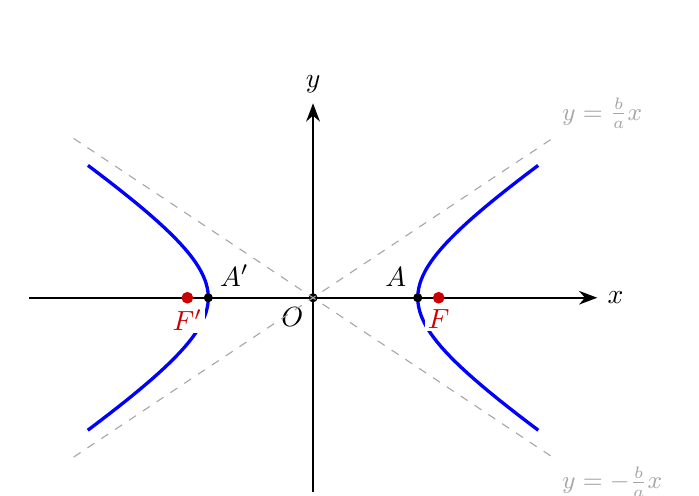
\begin{tikzpicture}[scale=0.95]
  \draw[thick, -Stealth] (-3.8, 0) -- (3.8, 0) node[right] {$x$};
  \draw[thick, -Stealth] (0, -2.6) -- (0, 2.6) node[above] {$y$};
  \filldraw (0, 0) circle (1.5pt) node[below left] {$O$};

  % Asymptotes
  \draw[dashed, gray!70] (-3.2, -2.13) -- (3.2, 2.13) node[above right] {\small $y = \frac{b}{a}x$};
  \draw[dashed, gray!70] (-3.2, 2.13) -- (3.2, -2.13) node[below right] {\small $y = -\frac{b}{a}x$};

  % Hyperbola branches (a=1.4, b=0.93)
  \draw[very thick, blue, domain=-1.4:1.4, samples=50] plot ({1.4*cosh(\x)}, {0.93*sinh(\x)});
  \draw[very thick, blue, domain=-1.4:1.4, samples=50] plot ({-1.4*cosh(\x)}, {0.93*sinh(\x)});

  % Foci c = sqrt(1.4^2 + 0.93^2) approx 1.68
  \filldraw[red!80!black] (1.68, 0) circle (2pt) node[below=3pt, fill=white, inner sep=1pt] {$F$};
  \filldraw[red!80!black] (-1.68, 0) circle (2pt) node[below=3pt, fill=white, inner sep=1pt] {$F'$};
  \filldraw (1.4, 0) circle (1.5pt) node[above left=1pt] {$A$};
  \filldraw (-1.4, 0) circle (1.5pt) node[above right=1pt] {$A'$};
\end{tikzpicture}
\caption{雙曲線與漸近線}
\label{fig:b4-2-1-9}
\end{figure}

取雙曲線之一葉與拋物線比較，它們的一個重要差異便是前者有漸近直線或簡稱漸近線，而後者沒有（§ III-3，丙）．如圖 \ref{fig:b4-2-1-9}，兩斜交直線卽為該雙曲線之漸近線，當點沿雙曲線向遠方伸展時，將與兩斜交直線無限接近．

其實拋物線也可看成雙曲線之極限情形．亦卽固定頂點 $A$，且固定一個焦點，讓另一焦點趨向遠處，則雙曲線逐漸退化成為拋物線，與圖 \ref{fig:b4-2-1-8} 合在一起，可得到下圖 \ref{fig:b4-2-1-10}：

\begin{figure}[H]
\centering
\begin{tikzpicture}[scale=1.05]
  \draw[thick, -Stealth] (-2.5, 0) -- (4.5, 0) node[right] {$x$};
  \draw[thick, -Stealth] (0, -2.5) -- (0, 2.5) node[above] {$y$};
  \filldraw (0, 0) circle (1.5pt) node[below left] {$A$};
  \filldraw (1, 0) circle (2pt) node[below=2pt, fill=white, inner sep=1pt] {$F$};

  % Ellipse sharing A and F
  \draw[thick, blue] (1.2, 0) ellipse (1.2 and 1.0);
  \node[blue] at (1.2, 1.25) {\small 橢圓};
  % Parabola sharing A and F
  \draw[very thick, green!60!black, domain=-2:2, samples=50] plot ({0.25*\x*\x}, \x);
  \node[green!60!black] at (2.4, 1.8) {\small 拋物線};
  % Hyperbola branch sharing A
  \draw[very thick, red, domain=-1.5:1.5, samples=50] plot ({0.7*(cosh(\x) - 1)}, {1.2*sinh(\x)});
  \node[red] at (3.4, 0.9) {\small 雙曲線};
\end{tikzpicture}
\caption{錐線系列演變：橢圓、拋物線、雙曲線之連續過渡}
\label{fig:b4-2-1-10}
\end{figure}
% =========================================================================
% § II-2 一個關於球的切線長度的事實
% =========================================================================
\subsection{一個關於球的切線長度的事實}
\label{sec:b4-2-2}

我們將用一固定圓錐與各種平面的截痕來引出所有可能的二次曲線，在這之前，先提及一個有用的事實：「球外一點到球的所有切線等長」．

取定空間的一個正交座標系 $S \equiv (O; \mathbf{e}_1, \mathbf{e}_2, \mathbf{e}_3)$，則空間中的點都可以用三個沿著一定秩序排成的實數 $x, y, z$ 來表示，亦卽，設點為 $P$，則因向量 $\vec{OP}$ 可表成
\[ \vec{OP} = x\mathbf{e}_1 + y\mathbf{e}_2 + z\mathbf{e}_3 = (x, y, z)_S \]
$P$ 與三數 $(x, y, z)_S$ 相互決定，而 $x, y, z$ 為 $\vec{OP}$ 的三個向量成分．這觀點第三冊已介紹過了．

\begin{figure}[H]
\centering
\begin{tikzpicture}[scale=0.9]
  \draw[thick, -Stealth] (0, 0) -- (3, 0) node[right] {$y$ ($\mathbf{e}_2$)};
  \draw[thick, -Stealth] (0, 0) -- (0, 3) node[above] {$z$ ($\mathbf{e}_3$)};
  \draw[thick, -Stealth] (0, 0) -- (-1.8, -1.8) node[below left] {$x$ ($\mathbf{e}_1$)};
  \filldraw (0, 0) circle (1.5pt) node[above left] {$O$};

  \coordinate (P) at (1.5, 1.8);
  \filldraw (P) circle (1.5pt) node[above right] {$P(x, y, z)$};
  \draw[very thick, -Stealth, blue] (0, 0) -- (P) node[midway, left] {$\vec{OP}$};
\end{tikzpicture}
\caption{空間正交座標系}
\label{fig:b4-2-2-1}
\end{figure}

球面是由所有到某一定點等距離的點組成，這定點常稱為球心，而球面上點到球心的距離稱為半徑．今空間中給定一半徑為 $r$ 的球面 $S$，若選一正交座標系 $S \equiv (O; \mathbf{e}_1, \mathbf{e}_2, \mathbf{e}_3)$ 使其基準點 $O$ 卽為球心，則空間中一點 $P = (x, y, z)_S$ 座落在這球面的充要條件為
\[ |\vec{OP}| = r \iff |\vec{OP}|^2 = r^2 \]
但根據畢氏定理 $|\vec{OP}|^2 = x^2 + y^2 + z^2$，故球面方程式為
\begin{equation}
x^2 + y^2 + z^2 = r^2 \label{eq:b4-2-2-1}
\end{equation}

設以 $S$ 表球面，引一直線 $L$，並取自 $Q(x_0, y_0, z_0)$ 沿 $L$ 的一個單位向量 $\mathbf{u} = (\cos\alpha, \cos\beta, \cos\gamma)$．

\begin{figure}[H]
\centering
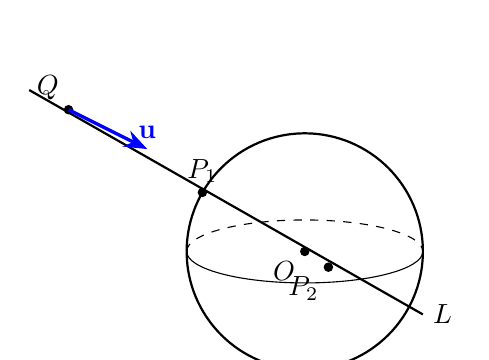
\begin{tikzpicture}[scale=1.0]
  % Sphere
  \draw[thick] (0, 0) circle (1.5);
  \draw[dashed] (-1.5, 0) arc (180:0:1.5 and 0.4);
  \draw (1.5, 0) arc (0:-180:1.5 and 0.4);
  \filldraw (0, 0) circle (1.5pt) node[below left] {$O$};

  % Secant Line L from Q
  \coordinate (Q) at (-3, 1.8);
  \coordinate (P1) at (-1.3, 0.75);
  \coordinate (P2) at (0.3, -0.2);
  \filldraw (Q) circle (1.5pt) node[above left] {$Q$};
  \filldraw (P1) circle (1.5pt) node[above] {$P_1$};
  \filldraw (P2) circle (1.5pt) node[below left] {$P_2$};
  \draw[thick] (-3.5, 2.05) -- (1.5, -0.8) node[right] {$L$};
  \draw[very thick, -Stealth, blue] (Q) -- (-2, 1.3) node[above] {$\mathbf{u}$};
\end{tikzpicture}
\caption{直線與球面相交}
\label{fig:b4-2-2-2}
\end{figure}

因此直線 $L$ 上的點 $M$ 皆可表成
\begin{align*}
\vec{OM} &= \vec{OQ} + \vec{QM} = \vec{OQ} + t\mathbf{u} \\
&= (x_0, y_0, z_0) + (t\cos\alpha, t\cos\beta, t\cos\gamma) \\
&= (x_0 + t\cos\alpha, \; y_0 + t\cos\beta, \; z_0 + t\cos\gamma)
\end{align*}
其中因 $\vec{QM} = t\mathbf{u}$，設 $L$ 上取一座標系 $S_L \equiv (Q; \mathbf{u})$，則 $t$ 可以看成 $M$ 點在 $L$ 上的 $S_L$---座標．

於是直線上點 $M$ 正好座落在球面 $S$ 上的充要條件為其座標滿足 \eqref{eq:b4-2-2-1} 式，亦卽
\[ (x_0 + t\cos\alpha)^2 + (y_0 + t\cos\beta)^2 + (z_0 + t\cos\gamma)^2 = r^2 \]
展開，依參數 $t$ 集項得
\[ t^2(\cos^2\alpha + \cos^2\beta + \cos^2\gamma) + 2t(x_0\cos\alpha + y_0\cos\beta + z_0\cos\gamma) + (x_0^2 + y_0^2 + z_0^2 - r^2) = 0 \]
又因 $\cos^2\alpha + \cos^2\beta + \cos^2\gamma = 1$，得
\begin{equation}
t^2 + 2(x_0\cos\alpha + y_0\cos\beta + z_0\cos\gamma)t + (x_0^2 + y_0^2 + z_0^2 - r^2) = 0 \label{eq:b4-2-2-2}
\end{equation}
這是一個 $t$ 的二次方程式，它最多有兩個實數根 $t_1$ 及 $t_2$．換句話說，直線 $L$ 最多與球面 $S$ 交於兩個點 $P_1$ 及 $P_2$．而這兩點 $P_1, P_2$ 的 $S_L$---座標分別為 $t_1, t_2$，亦卽 $\vec{QP_1} = t_1\mathbf{u}, \vec{QP_2} = t_2\mathbf{u}$．

注意因 $\mathbf{u}$ 為單位向量，$|t_1|$ 及 $|t_2|$ 正好代表 $Q$ 到 $P_1$ 與 $P_2$ 的距離，卽 $|t_1| = |QP_1|, |t_2| = |QP_2|$．

由 \eqref{eq:b4-2-2-2} 式之根與係數的關係，當 $Q$ 在球外，$P_1$ 與 $P_2$ 落在 $Q$ 的同側，$t_1$ 與 $t_2$ 同號，故此時
\begin{equation}
|QP_1| \cdot |QP_2| = t_1 t_2 = x_0^2 + y_0^2 + z_0^2 - r^2 = |\vec{OQ}|^2 - r^2 \label{eq:b4-2-2-3}
\end{equation}

\begin{definition}[定義]
空間中直線 $L$ 若與球面 $S$ 相交於兩點 $P_1$ 及 $P_2$，$L$ 稱為 $S$ 的割線．若只交於一點時，亦卽 $P_1$ 與 $P_2$ 重合時，$L$ 稱為 $S$ 的切線，或稱 $L$ 切於 $S$，此時 $L$ 上一點 $Q$ 到切點的距離稱為 $Q$ 到球面 $S$ 的切線長．
\end{definition}

當 $L$ 切於 $S$ 時，$P_1$ 與 $P_2$ 重合（稱切點 $P$），卽
\begin{equation}
|QP|^2 = |\vec{OQ}|^2 - r^2 \label{eq:b4-2-2-4}
\end{equation}
更因左端 $\ge 0$，故 $|\vec{OQ}|^2 - r^2 \ge 0$，知當 $L$ 切於球面時，$Q$ 不落在球的內部．進一步由廣義畢氏定理，\eqref{eq:b4-2-2-4} 式告訴我們 $\angle OPQ$ 成一直角，亦卽切線垂直於過切點的半徑．

歸結本節所述可得：

\begin{theorem}[定理 1（球的割線定理）]
空間中給定一點 $Q$ 及一以 $O$ 為心，以 $r$ 為半徑的球面 $S$，則過該點 $Q$ 的任一直線 $L$ 最多只能交球面於兩點 $P_1, P_2$，若 $L$ 上取一座標系 $S_L \equiv (Q; \mathbf{u})$，$P_1, P_2$ 的 $S_L$---座標分別為 $t_1, t_2$，則當 $Q$ 在球外，恆有
\[ |QP_1| \cdot |QP_2| = |\vec{OQ}|^2 - r^2 \]
\end{theorem}

\begin{theorem}[定理 1'（球的切線長定理）]
球外給定一點 $Q$ 到球的切線垂直於過切點的半徑，且所有這些切線等長，皆為定值：
\[ \sqrt{|\vec{OQ}|^2 - r^2} \]
其中 $O$ 為球心，$r$ 為球半徑．
\end{theorem}

\subsubsection*{習題 2-2}
\begin{enumerate}
  \item 求 $(4, 1, 1)$ 至球面 $(x+1)^2 + y^2 + (z-2)^2 = 16$ 的切線長．
  \item 設過點 $Q(3, 2, 1)$ 之直線 $L$ 與球面 $x^2 + y^2 + z^2 = 4$ 相交於 $P_1, P_2$ 兩點，求 $|QP_1| \cdot |QP_2|$ 之值．
  \item 求過點 $(0, 0, 0)$ 與直線 $\frac{x-1}{2} = \frac{y-2}{1} = \frac{z-3}{2}$ 上點到球面 $(x+1)^2 + y^2 + (z-2)^2 = 16$ 之交點．
  \item 試證：至二球面 $S_1, S_2$ 切線長相等的點的軌跡為一平面 $\pi$（$\pi$ 稱為二球面的根平面）．
\end{enumerate}

% =========================================================================
% § II-3 圓錐曲線
% =========================================================================
\subsection{圓錐曲線}
\label{sec:b4-2-3}

本章我們的用意是要從圓錐與平面的截痕（將稱為圓錐曲線或簡稱錐線）得到各種二次曲線；這節我們先直觀地來看各種圓錐曲線如何隨著截平面而演變．

\begin{definition}[定義]
所謂圓錐面便是在空間中，取定一平面及其上兩條相交於一點 $K$ 的直線 $L_0$ 及 $L_1$，然後以 $L_0$ 為固定軸將平面迴轉，此時，另一直線 $L_1$ 掃出一個錐狀的曲面，這樣得到的曲面便稱為圓錐面，設以 $\Omega$ 記之，$K$ 稱為圓錐 $\Omega$ 的頂點，$L_0$ 稱為 $\Omega$ 的中心軸，迴轉中的 $L_1$ 在任一時刻的位置是一條 $\Omega$ 上的直線，稱為 $\Omega$ 的一條母線．而 $L_0$ 與 $L_1$ 的夾角 $\omega$ 則稱圓錐的頂半角（此角為一定角，不隨 $L_1$ 的迴轉而改變）．
\end{definition}

\begin{figure}[H]
\centering
\begin{tikzpicture}[scale=0.9]
  % Cone apex
  \coordinate (K) at (0, 0);
  % Upper cone
  \draw[thick] (K) -- (-2, 3);
  \draw[thick] (K) -- (2, 3);
  \draw[thick] (0, 3) ellipse (2 and 0.5);
  % Lower cone
  \draw[thick] (K) -- (-2, -3);
  \draw[thick] (K) -- (2, -3);
  \draw[thick] (0, -3) ellipse (2 and 0.5);
  % Axis L0
  \draw[dashed, very thick] (0, -3.8) -- (0, 3.8) node[above] {$L_0$ (中心軸)};
  \filldraw (K) circle (2pt) node[right] {$K$ (頂點)};
  % Angle omega
  \draw (0, 1.2) arc (90:124:1.2) node[midway, above] {$\omega$};
\end{tikzpicture}
\caption{圓錐面及其組成要素}
\label{fig:b4-2-3-1}
\end{figure}

\begin{definition}[定義]
設 $\Omega$ 為一以 $K$ 為頂點的圓錐．一個不含 $K$ 的平面 $\pi$ 與 $\Omega$ 的截痕稱為圓錐曲線，或簡稱錐線．不妨將 $\Omega$ 固定使之正立，而中心軸 $L_0$ 鉛垂向上．當截平面 $\pi$ 交中心軸 $L_0$ 於一點 $M$ 時，取 $\pi$ 的一個單位法向量 $\mathbf{u} = \vec{MN}$ 使 $N$ 與頂點 $K$ 在 $\pi$ 的同側．取一平面 $\pi_0$ 含 $L_0$ 與 $MN$，稱法向量與中心軸的夾角 $\theta$ 為 $\pi$ 在 $\Omega$ 上的截角．當 $\pi$ 不與 $L_0$ 相交於一點時，定義截角 $\theta = \frac{\pi}{2}$．
\end{definition}

在介紹本題之前我們引入兩個直觀立體幾何的定理：

\begin{theorem}[定理 2]
設 $L_1$ 為平面 $\pi$ 的垂線，$\pi_1$ 為任意含 $L_1$ 的平面，交 $\pi$ 於直線 $L$，若自 $\pi_1$ 上一點 $P$ 引 $L$ 的垂線 $PN$（交 $L$ 於 $N$），則 $PN$ 亦為平面 $\pi$ 的垂線．
\end{theorem}

\begin{figure}[H]
\centering
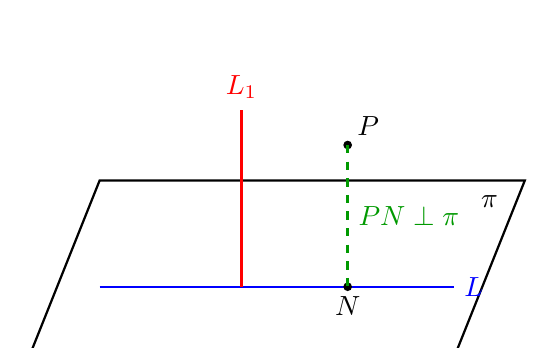
\begin{tikzpicture}[scale=0.9]
  % Plane pi
  \draw[thick] (-2, -1) -- (4, -1) -- (5, 1.5) -- (-1, 1.5) -- cycle;
  \node at (4.5, 1.2) {$\pi$};
  % Intersection line L
  \draw[thick, blue] (-1, 0) -- (4, 0) node[right] {$L$};
  % Perpendicular line L1
  \draw[very thick, red] (1, 0) -- (1, 2.5) node[above] {$L_1$};
  % Point P and PN
  \coordinate (P) at (2.5, 2);
  \coordinate (N) at (2.5, 0);
  \filldraw (P) circle (1.5pt) node[above right] {$P$};
  \filldraw (N) circle (1.5pt) node[below] {$N$};
  \draw[very thick, dashed, green!60!black] (P) -- (N) node[midway, right] {$PN \perp \pi$};
\end{tikzpicture}
\caption{定理 2 垂線性質示意圖}
\label{fig:b4-2-3-3}
\end{figure}

\begin{theorem}[定理 3（三垂線定理）]
設 $L$ 垂直於平面 $\pi$，垂足為 $M$，$L'$ 為 $\pi$ 上一直線，若自直線 $L$ 上一點 $P$ 引 $L'$ 的垂線（在由 $P$ 與 $L'$ 所決定的平面上引這垂線），垂足為 $N$，則 $MN \perp L'$．
\end{theorem}

\begin{figure}[H]
\centering
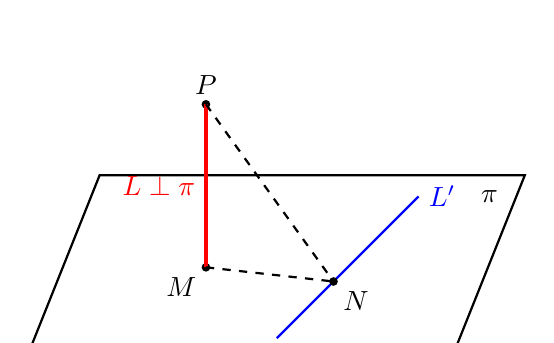
\begin{tikzpicture}[scale=0.9]
  % Plane pi
  \draw[thick] (-2, -1) -- (4, -1) -- (5, 1.5) -- (-1, 1.5) -- cycle;
  \node at (4.5, 1.2) {$\pi$};
  \coordinate (M) at (0.5, 0.2);
  \coordinate (P) at (0.5, 2.5);
  \filldraw (M) circle (1.5pt) node[below left] {$M$};
  \filldraw (P) circle (1.5pt) node[above] {$P$};
  \draw[very thick, red] (M) -- (P) node[midway, left] {$L \perp \pi$};

  % Line L' in pi
  \draw[thick, blue] (1.5, -0.8) -- (3.5, 1.2) node[right] {$L'$};
  \coordinate (N) at (2.3, 0);
  \filldraw (N) circle (1.5pt) node[below right] {$N$};

  \draw[thick, dashed] (P) -- (N);
  \draw[thick, dashed] (M) -- (N);
\end{tikzpicture}
\caption{三垂線定理示意圖}
\label{fig:b4-2-3-4}
\end{figure}

回到我們的本題：當圓錐面 $\Omega$ 固定，相應的圓錐曲線 $\Gamma$ 隨著截平面 $\pi$ 在 $\Omega$ 上的截角 $\theta$ 的變化而從正圓，橢圓，變成拋物線，再變為雙曲線．令 $\omega' = \frac{\pi}{2} - \omega$ 為母線與中心軸垂直面之夾角（頂半角的餘角）：
\begin{enumerate}[(i)]
  \item 當 $\theta$ 在 $0$ 與 $\omega'$ 之間（$0 \le \theta < \omega'$）時，截痕為“橢圓”模樣（特殊地當 $\theta = 0$ 時，截痕 $\Gamma$ 為正圓）．
  \item 當 $\theta = \omega'$ 時，截面與一條母線平行，截痕 $\Gamma$ 為拋物線模樣．
  \item 當 $\theta > \omega'$ 時，截面與圓錐兩葉皆相交，截痕 $\Gamma$ 擴大為兩葉，呈“雙曲線”形狀．
\end{enumerate}

\begin{figure}[H]
\centering
\begin{tikzpicture}[scale=0.85]
  % Three cone sections
  \begin{scope}[shift={(0, 0)}]
    \draw (-1.5, 2) -- (0, 0) -- (1.5, 2);
    \draw (-1.5, -2) -- (0, 0) -- (1.5, -2);
    \draw[blue, thick] (0, 1.2) ellipse (0.8 and 0.3);
    \node at (0, -2.5) {\small (i) $0 \le \theta < \omega'$（橢圓/圓）};
  \end{scope}

  \begin{scope}[shift={(4.5, 0)}]
    \draw (-1.5, 2) -- (0, 0) -- (1.5, 2);
    \draw (-1.5, -2) -- (0, 0) -- (1.5, -2);
    \draw[green!60!black, thick] (-0.8, 1.8) parabola bend (0.3, 0.4) (1.2, 1.8);
    \node at (0, -2.5) {\small (ii) $\theta = \omega'$（拋物線）};
  \end{scope}

  \begin{scope}[shift={(9.0, 0)}]
    \draw (-1.5, 2) -- (0, 0) -- (1.5, 2);
    \draw (-1.5, -2) -- (0, 0) -- (1.5, -2);
    \draw[red, thick] (-0.6, 1.8) parabola bend (0.2, 0.5) (0.8, 1.8);
    \draw[red, thick] (-0.6, -1.8) parabola bend (0.2, -0.5) (0.8, -1.8);
    \node at (0, -2.5) {\small (iii) $\theta > \omega'$（雙曲線）};
  \end{scope}
\end{tikzpicture}
\caption{圓錐截痕之分類演變}
\label{fig:b4-2-3-5}
\end{figure}

至於當截平面 $\pi$ 通過圓錐頂點 $K$ 時，在上述 (i), (ii), (iii) 的條件下，所得的截痕分別為一點、一直線或兩相交直線，稱為退化二次曲線．
% =========================================================================
% § II-4 焦半徑與離心率的觀點
% =========================================================================
\subsection{焦半徑與離心率的觀點}
\label{sec:b4-2-4}

現在我們要利用 § II-2 的球切線長定理，來導出圓錐截痕的焦點與焦半徑性質．這個精妙的幾何構想是 1822 年由比利時數學家丹德林（Dandelin）所發現的，稱為丹德林雙球定理．

\subsubsection*{甲、負類錐線（橢圓）}

在圓錐面 $\Omega$ 內放置兩個大小適當的球 $S$ 與 $S'$，使其分別與截平面 $\pi$ 相切於 $F$ 與 $F'$ 兩點，同時又與圓錐面 $\Omega$ 沿兩個水平圓周 $C_1$ 與 $C_2$ 相切（圖 \ref{fig:b4-2-4-1}）．這兩切點 $F$ 與 $F'$ 卽為錐線的兩個焦點．

\begin{figure}[H]
\centering
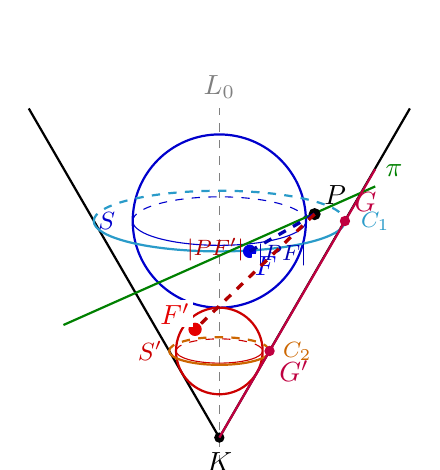
\begin{tikzpicture}[scale=1.1]
  % Cone outline
  \coordinate (K) at (0, 0);
  \draw[thick] (-2.2, 3.8) -- (K) -- (2.2, 3.8);
  \draw[dashed, gray] (0, -0.3) -- (0, 3.8) node[above] {$L_0$};
  \filldraw (K) circle (1.5pt) node[below=2pt] {$K$};

  % Sphere S (upper, larger)
  \coordinate (O1) at (0, 2.5);
  \draw[blue!80!black, thick] (O1) circle (1.0);
  \draw[blue!80!black, dashed] (-1.0, 2.5) arc (180:0:1.0 and 0.28);
  \draw[blue!80!black] (1.0, 2.5) arc (0:-180:1.0 and 0.28);
  \node[blue!80!black] at (-1.3, 2.5) {\small $S$};

  % Contact circle C1 where S touches the cone
  \draw[cyan!80!black, thick, dashed] (-1.45, 2.5) arc (180:0:1.45 and 0.35);
  \draw[cyan!80!black, thick] (1.45, 2.5) arc (0:-180:1.45 and 0.35);
  \node[cyan!80!black] at (1.8, 2.5) {\footnotesize $C_1$};

  % Sphere S' (lower, smaller)
  \coordinate (O2) at (0, 1.0);
  \draw[red!80!black, thick] (O2) circle (0.5);
  \draw[red!80!black, dashed] (-0.5, 1.0) arc (180:0:0.5 and 0.14);
  \draw[red!80!black] (0.5, 1.0) arc (0:-180:0.5 and 0.14);
  \node[red!80!black] at (-0.8, 1.0) {\small $S'$};

  % Contact circle C2 where S' touches the cone
  \draw[orange!80!black, thick, dashed] (-0.58, 1.0) arc (180:0:0.58 and 0.16);
  \draw[orange!80!black, thick] (0.58, 1.0) arc (0:-180:0.58 and 0.16);
  \node[orange!80!black] at (0.9, 1.0) {\footnotesize $C_2$};

  % Cutting plane pi
  \draw[thick, green!50!black] (-1.8, 1.3) -- (1.8, 2.9) node[above right] {$\pi$};
  \coordinate (F) at (0.35, 2.15);
  \coordinate (Fp) at (-0.28, 1.25);
  \filldraw[blue!90!black] (F) circle (2pt) node[below right=1pt, fill=white, inner sep=1pt] {$F$};
  \filldraw[red!90!black] (Fp) circle (2pt) node[above left=1pt, fill=white, inner sep=1pt] {$F'$};

  % Point P on ellipse
  \coordinate (P) at (1.1, 2.58);
  \filldraw (P) circle (1.8pt) node[above right] {$P$};

  % Generatrix KP cutting C1 at G and C2 at G'
  \coordinate (G) at (1.45, 2.5);
  \coordinate (Gp) at (0.58, 1.0);
  \draw[purple, thick] (K) -- (1.8, 3.1);
  \filldraw[purple] (G) circle (1.5pt) node[above right] {$G$};
  \filldraw[purple] (Gp) circle (1.5pt) node[below right] {$G'$};

  % Tangents from P to F and F'
  \draw[very thick, dashed, blue!70!black] (P) -- (F) node[midway, below] {\footnotesize $|PF|$};
  \draw[very thick, dashed, red!70!black] (P) -- (Fp) node[midway, above left] {\footnotesize $|PF'|$};
\end{tikzpicture}
\caption{丹德林雙球與橢圓焦半徑性質}
\label{fig:b4-2-4-1}
\end{figure}

設 $P$ 為截痕 $\Gamma$ 上的任意點，連結母線 $KP$，交圓 $C_1$ 於 $G$，交圓 $C_2$ 於 $G'$．因為直線 $PF$ 與 $PG$ 都是自點 $P$ 引至球 $S$ 的切線，由定理 1'，
\[ |PF| = |PG| \]
同理，直線 $PF'$ 與 $PG'$ 都是自點 $P$ 引至球 $S'$ 的切線，故
\[ |PF'| = |PG'| \]
相加得
\[ |PF| + |PF'| = |PG| + |PG'| = |GG'| \]
但線段 $GG'$ 夾在兩水平切圓 $C_1$ 與 $C_2$ 之間，其長度只決定於兩切圓間沿母線的距離，與點 $P$ 的選取完全無關！因此 $|GG'|$ 為一常數，記為 $2a$．

\begin{proposition}[命題 1（負類錐線焦半徑性質）]
對於負類錐線（橢圓）$\Gamma$ 上的任意點 $P$，恆有
\begin{equation}
|PF| + |PF'| = |GG'| = 2a = \text{定長} \label{eq:b4-2-4-1}
\end{equation}
\end{proposition}

\begin{corollary}[系理 1]
設截面交中心對稱平面於兩頂點 $A, A'$，則
\[ |AF| = |A'F'| \]
\end{corollary}

\begin{definition}[定義]
負類錐線（橢圓）的離心率定義為兩焦點距離與兩頂點距離之比：
\begin{equation}
e = \frac{|FF'|}{|AA'|} = \frac{2c}{2a} = \frac{c}{a} \label{eq:b4-2-4-ecc}
\end{equation}
因為兩焦點 $F, F'$ 落在頂點 $A, A'$ 內部，故恆有 $0 \le e < 1$．特別地，當截面水平時，$F = F'$ 重合為圓心，此時 $e = 0$（正圓）．
\end{definition}

\subsubsection*{乙、零類錐線（拋物線）}

當截角 $\theta = \omega'$ 時，截平面與圓錐的一條母線平行，此時只能在圓錐內放入一個與截面及圓錐相切的球 $S$（另一個球跑到無窮遠處），故拋物線只有一個焦點 $F$．離心率規定為 $e = 1$．

\begin{proposition}[命題 2]
拋物線可視為橢圓當另一焦點 $F'$ 趨向無窮遠處時之極限情況．
\end{proposition}

\subsubsection*{丙、正類錐線（雙曲線）}

當截角 $\theta > \omega'$ 時，截面與圓錐的上下兩葉皆相交，截痕為雙曲線．此時丹德林雙球分別位於圓錐頂點 $K$ 的兩側：一個在頂點上葉內切於球 $S$，切點為 $F$；另一個在頂點下葉內切於球 $S'$，切點為 $F'$（圖 \ref{fig:b4-2-4-7}）．

\begin{figure}[H]
\centering
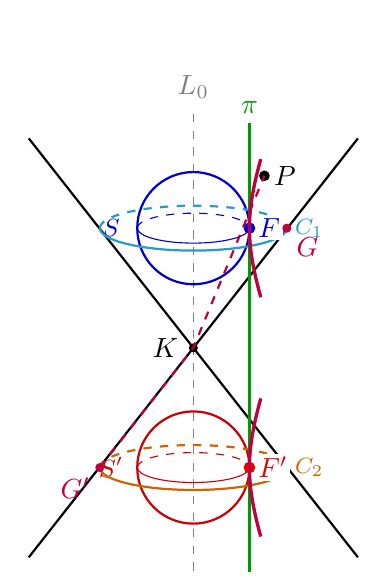
\begin{tikzpicture}[scale=0.95]
  % Double cone outline
  \coordinate (K) at (0, 0);
  \draw[thick] (-2.2, 2.8) -- (K) -- (2.2, 2.8);
  \draw[thick] (-2.2, -2.8) -- (K) -- (2.2, -2.8);
  \draw[dashed, gray] (0, -3.2) -- (0, 3.2) node[above] {$L_0$};
  \filldraw (K) circle (1.5pt) node[left=2pt] {$K$};

  % Sphere in upper cone S
  \coordinate (O1) at (0, 1.6);
  \draw[blue!80!black, thick] (O1) circle (0.75);
  \draw[blue!80!black, dashed] (-0.75, 1.6) arc (180:0:0.75 and 0.2);
  \draw[blue!80!black] (0.75, 1.6) arc (0:-180:0.75 and 0.2);
  \node[blue!80!black] at (-1.1, 1.6) {\small $S$};

  % Contact circle C1
  \draw[cyan!80!black, thick, dashed] (-1.25, 1.6) arc (180:0:1.25 and 0.3);
  \draw[cyan!80!black, thick] (1.25, 1.6) arc (0:-180:1.25 and 0.3);
  \node[cyan!80!black] at (1.55, 1.6) {\footnotesize $C_1$};

  % Sphere in lower cone S'
  \coordinate (O2) at (0, -1.6);
  \draw[red!80!black, thick] (O2) circle (0.75);
  \draw[red!80!black, dashed] (-0.75, -1.6) arc (180:0:0.75 and 0.2);
  \draw[red!80!black] (0.75, -1.6) arc (0:-180:0.75 and 0.2);
  \node[red!80!black] at (-1.1, -1.6) {\small $S'$};

  % Contact circle C2
  \draw[orange!80!black, thick, dashed] (-1.25, -1.6) arc (180:0:1.25 and 0.3);
  \draw[orange!80!black, thick] (1.25, -1.6) arc (0:-180:1.25 and 0.3);
  \node[orange!80!black] at (1.55, -1.6) {\footnotesize $C_2$};

  % Cutting plane pi
  \draw[thick, green!60!black] (0.75, -3.0) -- (0.75, 3.0) node[above] {$\pi$};
  \coordinate (F) at (0.75, 1.6);
  \coordinate (Fp) at (0.75, -1.6);
  \filldraw[blue!90!black] (F) circle (2pt) node[right=2pt, fill=white, inner sep=1pt] {$F$};
  \filldraw[red!90!black] (Fp) circle (2pt) node[right=2pt, fill=white, inner sep=1pt] {$F'$};

  % Hyperbolic branches on plane pi
  \draw[very thick, purple, domain=-0.9:0.9, samples=40] plot ({0.75 + 0.35*(cosh(\x)-1)}, {1.6 + 0.9*sinh(\x)});
  \draw[very thick, purple, domain=-0.9:0.9, samples=40] plot ({0.75 + 0.35*(cosh(\x)-1)}, {-1.6 - 0.9*sinh(\x)});

  % Point P and generatrix KP
  \coordinate (P) at (0.95, 2.3);
  \filldraw (P) circle (1.8pt) node[right] {$P$};
  \coordinate (G) at (1.25, 1.6);
  \coordinate (Gp) at (-1.25, -1.6);
  \draw[thick, dashed, purple] (Gp) -- (K) -- (P);
  \filldraw[purple] (G) circle (1.5pt) node[below right] {$G$};
  \filldraw[purple] (Gp) circle (1.5pt) node[below left] {$G'$};
\end{tikzpicture}
\caption{雙曲線之丹德林雙球模型}
\label{fig:b4-2-4-7}
\end{figure}

對雙曲線上任意點 $P$，同理由球切線等長定理：
\[ ||PF| - |PF'|| = |GG'| = 2a = \text{定長} \]

\begin{proposition}[命題 3（正類錐線焦半徑性質）]
對於正類錐線（雙曲線）上的任意點 $P$，恆有
\begin{equation}
||PF| - |PF'|| = 2a = \text{定長} \label{eq:b4-2-4-hyp}
\end{equation}
\end{proposition}

\begin{definition}[定義]
正類錐線（雙曲線）的離心率定義為
\begin{equation}
e = \frac{|FF'|}{|AA'|} = \frac{c}{a} > 1 \label{eq:b4-2-4-hyp-ecc}
\end{equation}
\end{definition}

\subsubsection*{習題 2-4}
\begin{enumerate}
  \item 參照圖 \ref{fig:b4-2-4-1} 與圖 \ref{fig:b4-2-4-7}，說明離心率其實是二球 $S, S'$ 的外公切線長與內公切線長的比．
  \item 設截平面在圓柱面（圓筒面）上的截痕為 $\Gamma$，試證 $\Gamma$ 亦有類似負類錐線的焦半徑性質．
\end{enumerate}

% =========================================================================
% § II-5 準線觀點
% =========================================================================
\subsection{\texorpdfstring{$\ddagger$ }{‡ }準線觀點}
\label{sec:b4-2-5}

設 $\Gamma$ 為截平面 $\pi$ 與圓錐面 $\Omega$ 的截痕，$\omega$ 為頂半角，$\theta$ 為截角，$\omega' = \frac{\pi}{2} - \omega$ 為其餘角．沿用上節符號，考慮切於圓錐與平面 $\pi$ 的丹德林球 $S$，切圓錐於小圓 $C_1$．設包含 $C_1$ 的水平面為 $\pi_1$，則 $\pi_1$ 與截平面 $\pi$ 相交於一直線 $p$，稱直線 $p$ 為錐線 $\Gamma$ 相應於焦點 $F$ 的一條準線．

\begin{figure}[H]
\centering
\begin{tikzpicture}[scale=1.1]
  % Cone outline
  \coordinate (K) at (0, 0);
  \draw[thick] (-2.2, 3.5) -- (K) -- (2.2, 3.5);
  \draw[dashed, gray] (0, -0.2) -- (0, 3.5) node[above] {$L_0$};
  \filldraw (K) circle (1.5pt) node[below=2pt] {$K$};

  % Sphere S and contact circle C1
  \coordinate (O1) at (0, 1.8);
  \draw[blue!80!black, thick] (O1) circle (0.8);
  \draw[blue!80!black, dashed] (-0.8, 1.8) arc (180:0:0.8 and 0.22);
  \draw[blue!80!black] (0.8, 1.8) arc (0:-180:0.8 and 0.22);

  % Horizontal plane pi1 (containing C1)
  \draw[cyan!60!black, thick] (-2.2, 1.8) -- (2.2, 1.8) node[right] {$\pi_1$ (含 $C_1$)};
  \draw[cyan!80!black, thick, dashed] (-1.13, 1.8) arc (180:0:1.13 and 0.28);
  \draw[cyan!80!black, thick] (1.13, 1.8) arc (0:-180:1.13 and 0.28);
  \node[cyan!80!black] at (1.4, 1.8) {\footnotesize $C_1$};

  % Cutting plane pi and directrix line p = pi cap pi1
  \draw[thick, green!50!black] (-1.6, 0.9) -- (1.8, 2.8) node[above right] {$\pi$};
  \coordinate (pLine) at (-0.6, 1.8);
  \filldraw[purple] (pLine) circle (2pt) node[above left=1pt, fill=white, inner sep=1pt] {$p$ (準線)};

  % Focus F
  \coordinate (F) at (0.35, 1.85);
  \filldraw[blue!90!black] (F) circle (2pt) node[below=3pt, fill=white, inner sep=1pt] {$F$};

  % Point P on section curve
  \coordinate (P) at (1.2, 2.45);
  \filldraw (P) circle (1.8pt) node[above right] {$P$};

  % Generatrix KP cutting C1 at G
  \coordinate (G) at (1.13, 1.8);
  \draw[thick, purple] (K) -- (P);
  \filldraw[purple] (G) circle (1.5pt) node[below right] {$G$};

  % Perpendicular PR to plane pi1
  \coordinate (R) at (1.2, 1.8);
  \draw[very thick, dashed, orange!80!black] (P) -- (R) node[midway, right] {\footnotesize $PR \perp \pi_1$};
  \filldraw[orange!80!black] (R) circle (1.5pt) node[below=2pt] {$R$};

  % Perpendicular PT to directrix p
  \coordinate (T) at (-0.6, 1.8);
  \draw[very thick, dashed, red!80!black] (P) -- (T) node[midway, above] {\footnotesize $PT \perp p$};
  \draw[thick, dashed, gray] (R) -- (T);

  % Tangent PF
  \draw[thick, dashed, blue!70!black] (P) -- (F) node[midway, below] {\footnotesize $PF$};
\end{tikzpicture}
\caption{錐線之準線與焦點幾何構造}
\label{fig:b4-2-5-1}
\end{figure}

設 $P$ 為 $\Gamma$ 上任一點，自 $P$ 引水平面 $\pi_1$ 的垂線，垂足為 $R$；自 $P$ 引準線 $p$ 的垂線，垂足為 $T$．可證得：
\[ |PG| = \frac{|PR|}{\cos\omega} = \frac{|PR|}{\sin\omega'}, \qquad |PT| = \frac{|PR|}{\sin\theta} \]
故
\[ \frac{|PF|}{|PT|} = \frac{|PG|}{|PT|} = \frac{\sin\theta}{\sin\omega'} = \text{定值} \]

\begin{theorem}[定理 4（準線性質）]
設 $\Gamma$ 為一般錐線，則 $\Gamma$ 上的點 $P$ 到焦點之距離 $|PF|$ 與到準線之距離 $|PT|$ 為一定比，且此比值正好等於離心率 $e$：
\begin{equation}
\frac{|PF|}{|PT|} = \frac{\sin\theta}{\sin\omega'} = e \label{eq:b4-2-5-1}
\end{equation}
\end{theorem}

在平面 $\pi$ 上建立正交座標系，以頂點連線之中點為原點，焦點在 $X$ 軸上，則有：
\begin{enumerate}[(i)]
  \item \textbf{橢圓（$0 < e < 1$）}：兩準線位於兩頂點外側，方程式為
  \begin{equation}
  x = \pm \frac{a^2}{c} = \pm \frac{a}{e} \label{eq:b4-2-5-ell-dir}
  \end{equation}
  \item \textbf{雙曲線（$e > 1$）}：兩準線位於兩頂點內側，方程式為
  \begin{equation}
  x = \pm \frac{a^2}{c} = \pm \frac{a}{e} \label{eq:b4-2-5-hyp-dir}
  \end{equation}
  \item \textbf{拋物線（$e = 1$）}：準線方程式為
  \begin{equation}
  x = -c \label{eq:b4-2-5-par-dir}
  \end{equation}
\end{enumerate}

\begin{figure}[H]
\centering
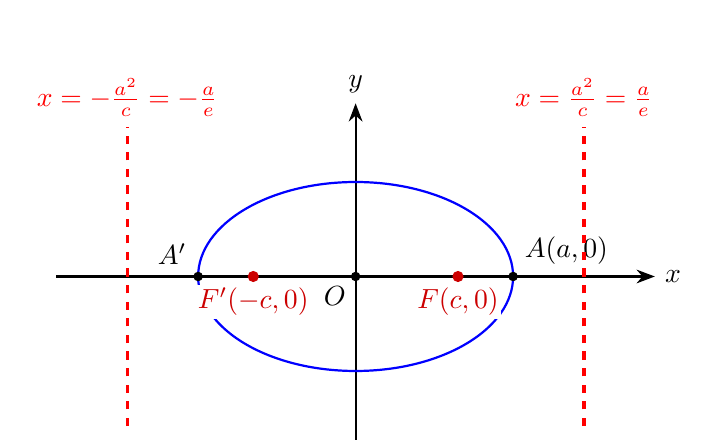
\begin{tikzpicture}[scale=1.0]
  \draw[thick, -Stealth] (-3.8, 0) -- (3.8, 0) node[right] {$x$};
  \draw[thick, -Stealth] (0, -2.2) -- (0, 2.2) node[above] {$y$};
  \filldraw (0, 0) circle (1.5pt) node[below left] {$O$};

  \draw[thick, blue] (0, 0) ellipse (2.0 and 1.2);
  \filldraw[red!80!black] (1.3, 0) circle (1.8pt) node[below=3pt, fill=white, inner sep=1pt] {$F(c, 0)$};
  \filldraw[red!80!black] (-1.3, 0) circle (1.8pt) node[below=3pt, fill=white, inner sep=1pt] {$F'(-c, 0)$};
  \filldraw (2.0, 0) circle (1.5pt) node[above right=1pt] {$A(a, 0)$};
  \filldraw (-2.0, 0) circle (1.5pt) node[above left=1pt] {$A'$};

  % Directrices
  \draw[very thick, dashed, red] (2.9, -1.9) -- (2.9, 1.9) node[above] {$x = \frac{a^2}{c} = \frac{a}{e}$};
  \draw[very thick, dashed, red] (-2.9, -1.9) -- (-2.9, 1.9) node[above] {$x = -\frac{a^2}{c} = -\frac{a}{e}$};
\end{tikzpicture}
\caption{橢圓之焦點與準線位置}
\label{fig:b4-2-5-4}
\end{figure}

\subsubsection*{習題 2-5}
\begin{enumerate}
  \item 是否平面在圓筒面（圓柱面）上的截痕亦有類似於錐線的定理 4 的準線性質？試繪立體圖，表明其準線位置，並求其離心率與截角關係．
  \item 比較圖 \ref{fig:b4-2-1-8} 與圖 \ref{fig:b4-2-1-10}，其區別為前者同時固定頂點 $A$ 與兩焦點之一，後者則只固定 $A$，而讓兩焦點間距離改變．
  \begin{enumerate}[(i)]
    \item 有否方法在一固定圓錐上取截平面使截痕的一個焦點向頂點無限逼近？
    \item 欲得到一系列錐線使其中一個焦點與一個頂點距離固定，應如何調整截平面？
  \end{enumerate}
\end{enumerate}

\vspace{1.5em}
\noindent\textbf{**〔章末附註〕}\phantomsection\label{note:b4-ch2-p96-appendix-note}

\textbf{定理 4 證明的幾何補充（$AM \perp p$ 證明）}：

自 $A$ 引 $\pi_1$ 的垂線交 $\pi_1$ 於 $R'$，再自 $R'$ 引直線 $AM$ 的垂線，垂足為 $B$．則因 $BR'$ 與 $MN$ 都垂直於 $MA$，且都在平面 $\pi_0$ 上，故 $BR' \parallel MN$．但 $MN$ 垂直於 $\pi$，故 $BR'$ 亦為 $\pi$ 的垂線．

另一方面，分別在 $\pi_1, \pi$ 上過 $R', A$ 引 $p$ 的平行直線 $l', l$，則因 $AR'$ 垂直於 $\pi_1$，故亦垂直於 $l'$，但 $l' \parallel l$，故 $AR'$ 亦垂直於 $l$．今利用三垂線定理得 $BA \perp l$，亦卽 $AM \perp p$．證畢．


\end{document}
